\subsection{Umsetzung der GUI im Code}\label{tkintercode}
\paragraph{Klassenstruktur}
Im Vordergrund basiert die Klassenstruktur grundsätzlich auf \gls{gls_ctk} Komponenten (siehe Abb.~\ref{fig:klassenstruktur_frontend}). Dabei gibt es die Klassen \enquote{App}, \enquote{PageFrame}, \enquote{TitleFrame} und \enquote{MeasurementFrame}. Im Programm wird eine \enquote{App} Instanz ausgeführt, welche das Hauptfenster ist. Diese Instanz kann beliebig viele \enquote{PageFrames} enthalten, die wiederum jeweils ein \enquote{TitleFrame} und eine Liste von \enquote{MeasurementFrames} beinhalten. Die \enquote{PageFrames} stellen die einzelnen Seiten dar, welche per Knopfdruck an der \acs{rltanzeige} durchgeblättert werden können. In einem \enquote{TitleFrame} wird immer der Titel der jeweiligen Seite gespeichert \bzw angezeigt. In den \enquote{MeasurementFrame} Instanzen werden hingegen die tatsächlichen Messwerte (Bezeichnung + Wert + Maßeinheit) dargestellt.

\begin{figure}[H]
	\centering
	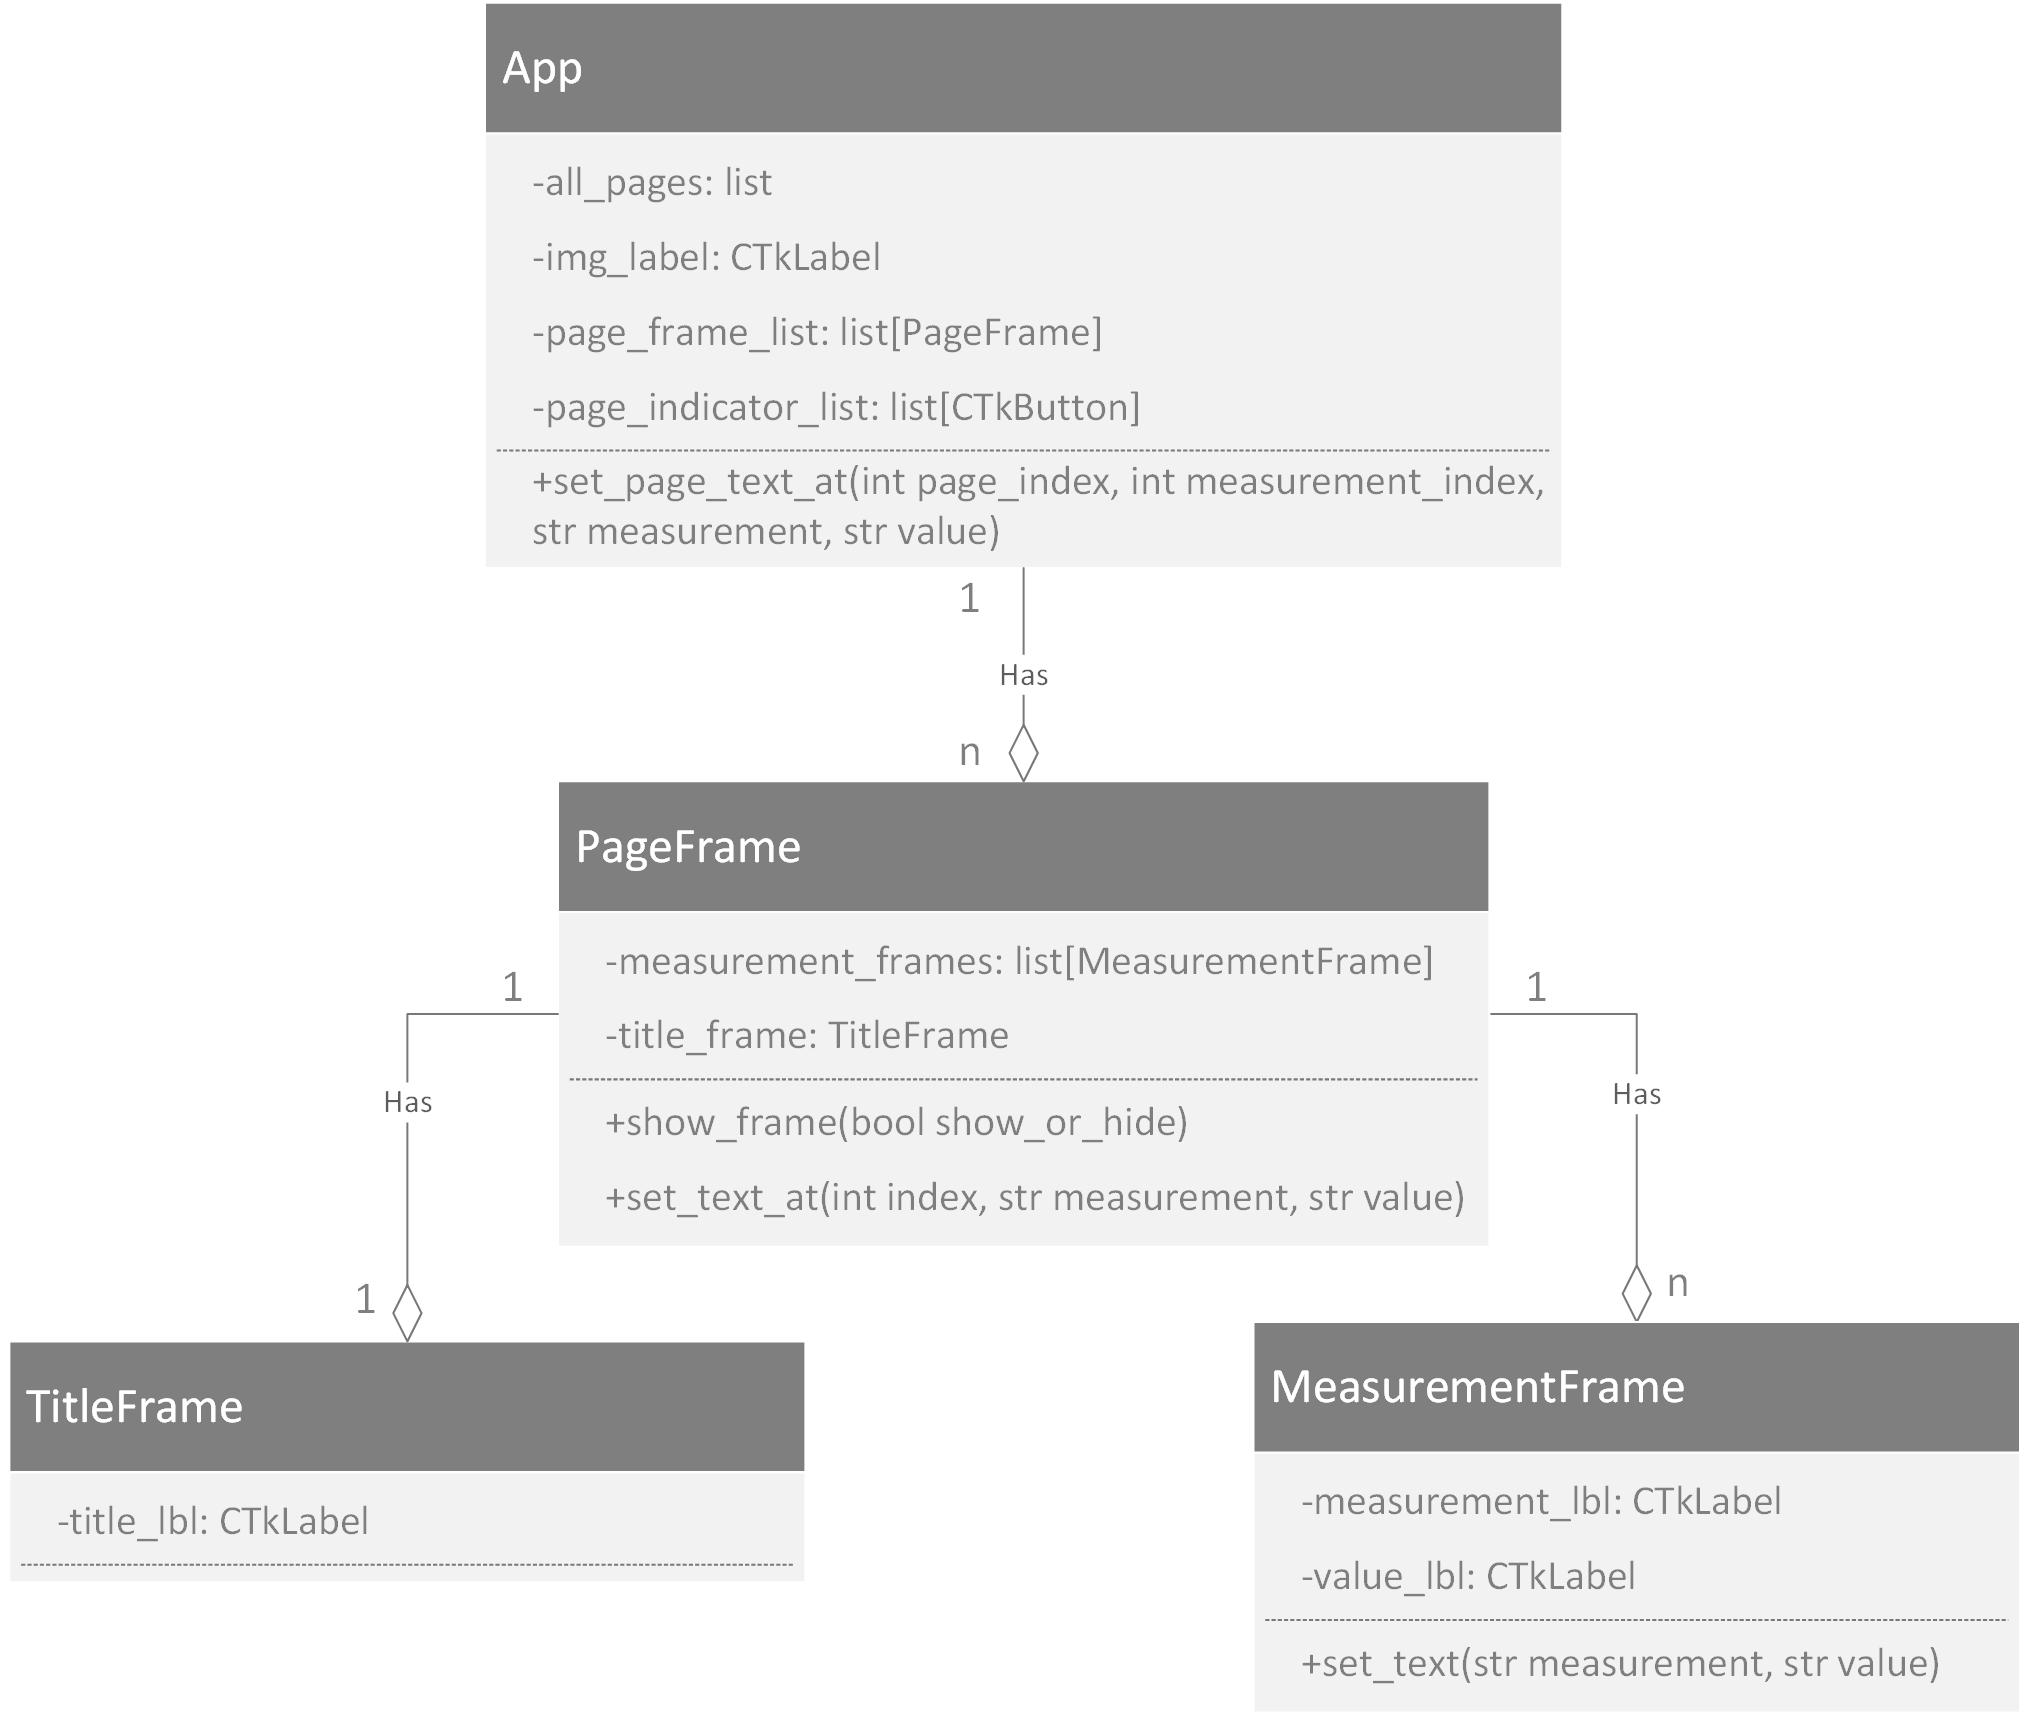
\includegraphics[width=0.84\textwidth]{uml_frontent_class_diagram}
	\caption{UML Diagramm Frontend \label{fig:klassenstruktur_frontend}}
\end{figure}

\paragraph{CustomTkinter Code}
Eine nähere Beschreibung und die Umsetzung der vorher genannten Klassen erfolgt in diesem Kapitel. 
\newline Wie zuletzt beschrieben, basieren alle Klassen im Frontend auf \gls{gls_ctk}. Die Klassen sind dabei alle (bis auf die Klasse \enquote{App}) vom Typen \enquote{CTkFrame}. Ein \enquote{CTkFrame} ist ein Widget, das wie ein Rahmen \bzw Behälter für andere Widgets fungiert. So können diese weiteren Widgets gruppiert und besser organisiert werden. Als erster Parameter wird für \enquote{CTkFrames}, wie bei allen \gls{gls_tk} und \gls{gls_ctk} Widgets, der \enquote{master} \bzw das Elternobjekt angegeben. Darüber hinaus können die Breite (\enquote{width}), Höhe (\enquote{height}), Rahmenbreite \bzw -Farbe (\enquote{border\_width} \bzw \enquote{border\_color}) sowie die Hintergrundfarbe (\enquote{fg\_color}) angegeben werden. \cite[vgl.][]{Schimansky:o.J.}

Die Klasse \enquote{TitleFrame} enthält ein \enquote{CTkLabel}, welches mit der \enquote{place( )} Methode im Behälter platziert wird. Die Klasse \enquote{CTkLabel} basiert auf der Klasse \enquote{tkinter.Label} und dient zur Darstellung eines Textes. In diesem Label steht immer der Titel der zugehörigen Seite. Das \enquote{title\_font} Objekt, welches im folgenden Code zu sehen ist, ist eine Instanz der \gls{gls_ctk} Utility Klasse \enquote{CTkFont}. Es wird verwendet um die Schriftformatierung von \gls{gls_ctk} Widgets vorzunehmen. Jedes \gls{gls_ctk} Widget bekommt standardmäßig ein \enquote{CTkFont} Objekt, wobei ein solches Objekt zeitgleich mehreren Widgets angefügt werden kann. Eine Änderung eines \enquote{CTkFont} Objekts wird an alle Widgets, die es verwenden, weitergeleitet. \cite[vgl.][]{Schimansky:o.J.}

\begin{pythoncode}
class TitleFrame(ctk.CTkFrame):
	def __init__(self, master, title, **kwargs):
		super().__init__(master, width=800, height=60, fg_color=text_color, **kwargs)
		
		title_font = ctk.CTkFont(family="Roboto", size=32)
		
		self.title_lbl = ctk.CTkLabel(master=self, text=title, width=700, height=45, fg_color="transparent", text_color=title_color, anchor=ctk.CENTER, font=title_font)
		self.title_lbl.place(relx=0.5, rely=0.12, anchor=ctk.N)
\end{pythoncode}

Wie in der Klassenstruktur beschrieben, beinhaltet ein jedes \enquote{PageFrame} neben einem \enquote{TitleFrame} eine Liste von \enquote{MeasurementFrames}. Eine Instanz der Klasse \enquote{MeasurementFrame} enthält immer Informationen zu einem bestimmten Messwert, welche mithilfe von zwei \enquote{CTkLabel} Widgets dargestellt werden. Dabei wird die Bezeichnung des Messwerts links im \enquote{measurement\_lbl} und der tätsichliche Wert einschließlich Maßeinheit rechts im \enquote{value\_lbl} platziert. Die zwei Labels werden durch einen Strich getrennt, der mit dem \gls{gls_tk} Widget \enquote{Canvas} erstellt wird. Ein Canvas ist ein rechteckiger Bereich \bzw eine Leinwand, auf dem Bilder oder andere komplexe Layouts gezeichnet werden können. Zusätzlich lassen sich auf einem Canvas Widget \zB weitere Widgets, Text oder Bilder platzieren. \cite[vgl.][20]{Shipman:2013} 
\newline Da jeder Messwert kontinuierlich aktualisiert wird, verfügt die \enquote{MeasurementFrame} über die Methode \enquote{set\_text}. In dieser wird mithilfe der \enquote{configure( )} Methode der Text beider Labels aktualisiert. Ein gekürzter Code zur \enquote{MeasurementFrame} Klasse folgt.

\begin{pythoncode}
class MeasurementFrame(ctk.CTkFrame):
	def __init__(self, master, measurement, value, **kwargs):
		#[Initialisierung des CTkFrames + Erstellung eines CTkFont Objekts zur Schriftformatierung der MeasurementFrames]
		
		self.measurement_lbl = ctk.CTkLabel(master=self, text=measurement, ...)
		self.value_lbl = ctk.CTkLabel(master=self, text=value, ...)
		self.canvas = Canvas(master=self, ...)
		#[Platzierung beider Labels + Canvas]
		
	def set_text(self, value):
		self.value_lbl.configure(text=value)
\end{pythoncode}

Die letzte der \gls{gls_ctk} \enquote{CTkFrame} Klassen ist die \enquote{PageFrame} Klasse. Wie bereits erwähnt dient jede Instanz dieser Klasse als unsichtbarer Behälter \bzw Seite, die ein \enquote{TitleFrame} sowie eine Liste von \enquote{MeasurementFrames} beinhält. Diese Komponenten werden, wie im nachstehenden Code zu sehen ist, im Konstruktor eines jeden \enquote{PageFrames} zugeordnet. Die Parameter \enquote{title} und \enquote{measurement} stammen aus der JSON Haupt-Konfigurationsdatei (siehe Kapitel \ref{json_config_files}, Tab. \ref{tab:pages_array_parameter} unter \enquote{title} \bzw Tab. \ref{tab:sources_array_parameter}  unter \enquote{description}) und können daher schon bei Erstellung der \enquote{PageFrame} Instanzen übergeben werden. Der \enquote{value} Parameter der individuellen \enquote{MeasurementFrames} hingegen wird laufend von der Methode \enquote{set\_text\_at( )} aktualisiert und ist daher am Anfang bis zum ersten Auslesen auf \enquote{N/A} (\dt nicht verfügbar) gesetzt.
	
\begin{pythoncode}
class PageFrame(ctk.CTkFrame):
	def __init__(self, master, title, parameters, **kwargs):
		#[Initialisierung des CTkFrames]
		self.measurement_frames = []
		self.title_frame = TitleFrame(master=master, title=title, ...)
		
		for parameter in parameters:
			frame = MeasurementFrame(master=master, measurement=parameter.description, value="N/A", ...)
			self.measurement_frames.append(frame)

    def set_text_at(self, index, value):
        self.measurement_frames[index].set_text(value)
...
\end{pythoncode}

Die \enquote{PageFrame} Klasse enthält zudem eine \enquote{show\_frame( )} Methode, die dazu dient die jeweilige \enquote{PageFrame} Instanz \bzw ihren Inhalt sichtbar oder unsichtbar zu machen. Diese Methode ist notwendig, damit zwischen den unterschiedlichen Seiten gewechselt werden kann.

\begin{pythoncode}
...
	def show_frame(self, show_or_hide):
		if show_or_hide:
			self.title_frame.place(...)
			self.title_frame.tkraise()
		else:
			self.title_frame.place_forget()
		
		for my_frame in self.measurement_frames:
			if show_or_hide:
				my_frame.place(...)
				my_frame.tkraise()
			else:
				my_frame.place_forget()
\end{pythoncode}

Die Klasse \enquote{App} 
Die \enquote{set\_page\_text\_at( )} Methode wird in der \enquote{data\_refresh( )} Methode aufgerufen (siehe Kapitel \ref{auslesen_rlt_parameter}), welche dazu dient, die Messwerte regelmäßig zu aktualisieren.

\begin{pythoncode}
class App(ctk.CTk):
	def __init__(self, all_pages, *args, **kwargs):
		super().__init__(*args, **kwargs)
		self.attributes('-fullscreen', True)
		self.resizable(False, False)
		self.config(cursor="none")
		
		boesch_logo = ctk.CTkImage(light_image=Image.open("..."), dark_image=Image.open("..."), size=(230, 230 * (1 / 3)))
		
		self.img_label = ctk.CTkLabel(master=self, image=boesch_logo, text="")
		self.img_label.place(...)
		
		global page_frame_list
		page_frame_list = []
		global page_indicator_list
		page_indicator_list = []
		
		for page in all_pages:  # Creates Frames based on the sensor data
			page_frame_list.append(PageFrame(master=self, title=page.title, parameters=page.measurements))
		
		page_frame_list[globals_.current_page].show_frame(True)

		start_x_position = 0.975 - len(page_frame_list) / 45.0
		
		if len(page_frame_list) > 1:
			for i in range(0, len(page_frame_list)):
				page_indicator_list.append(ctk.CTkButton(master=self, width=15, height=15, text="", corner_radius=50, fg_color=("#898989" if i == globals_.current_page else "#D9D9D9")))
				page_indicator_list[i].place(relx=start_x_position + i / 45.0, rely=0.93, anchor=ctk.CENTER)
		
	def set_page_text_at(self, page_index, measurement_index, value):
    	page_frame_list[page_index].set_text_at(measurement_index, value)
	
\end{pythoncode}
